%% The first command in your LaTeX source must be the \documentclass command.
%%
%% Options:
%% twocolumn : Two column layout.
%% hf: enable header and footer.
\documentclass[
% twocolumn,
% hf,
]{ceurart}


%%
%% Reviewing packages and definitions
\usepackage[dvipsnames,svgnames]{xcolor} % text color
\usepackage[normalem]{ulem} % wavy underlines
\newcommand{\todo}[1]{\noindent\textcolor{red}{{\bf \{TODO}: #1{\bf \}}}}
\newcommand{\TODO}[1]{\todo{#1}}
\newcommand{\citeneeded}{\textcolor{red}{{\bf [?!]}}}
\newenvironment{draft}{\color{gray}}{\color{black}}
\newcommand\jr[1]{{\color{Red}\textbf{JR}: #1}}

%%
%% One can fix some overfulls
\sloppy

%%
%% Minted listings support 
%% Need pygment <http://pygments.org/> <http://pypi.python.org/pypi/Pygments>
\usepackage[outputdir=build]{minted}
%% auto break lines
\setminted{breaklines=true}

%%
%% end of the preamble, start of the body of the document source.
\begin{document}

%%
%% Rights management information.
%% CC-BY is default license.
\copyrightyear{2022}
\copyrightclause{Copyright for this paper by its authors.
  Use permitted under Creative Commons License Attribution 4.0
  International (CC BY 4.0).}

%%
%% This command is for the conference information
\conference{Woodstock'22: Symposium on the irreproducible science,
  June 07--11, 2022, Woodstock, NY}

%%
%% The "title" command
\title{Bringing IDE Support to JSON-LD with the Language Server Protocol}

% \tnotemark[1]
% \tnotetext[1]{You can use this document as the template for preparing your
%   publication. We recommend using the latest version of the ceurart style.}

%%
%% The "author" command and its associated commands are used to define
%% the authors and their affiliations.
\author[1]{Arthur Vercruysse}[%
orcid=0000-0002-0877-7063,
email=arthur.vercruysse@ugent.be,
]
\author[1]{Julián Andrés Rojas}[%
orcid=0000-0002-0877-7063,
email=JulianAndres.RojasMelendez@UGent.be,
]
\author[1]{Pieter Colpaert}[%
orcid=0000-0001-7116-9338,
email=pieter.colpaert@ugent.be,
]
\cormark[1]
\fnmark[1]
\address[1]{IDLab, Department of Electronics and Information Systems, Ghent University – imec}
% \address[2]{IDLab, Department of Electronics and Information Systems, Ghent University – imec}
% \address[3]{IDLab, Department of Electronics and Information Systems, Ghent University – imec}

%% Footnotes
\cortext[1]{Corresponding author.}
\fntext[1]{These authors contributed equally.}

%%
%% The abstract is a short summary of the work to be presented in the
%% article.
\begin{abstract}
  JSON-LD is a popular data format used to describe and share semantic data on the web.
  However, creating and editing JSON-LD documents can be a challenging task, especially when dealing with complex (sometimes remote) contexts that include many properties.
  The existing JSON editing functionality may not suffice for developers, and a JSON-LD editor could greatly enhance their experience.
  In this paper, we introduce a JSON-LD Language Server Protocol (LSP) that enables text editors compatible with the LSP protocol (e.g., Visual Studio Code and NeoVim), to suggest autocompletion items based on the defined context, and it also enables renaming identifiers inside the document.
  We believe that the implementation of a JSON-LD LSP will enhance developer ergonomics and promote its adoption.
  Moreover, we see high potential for additional features that can be added such as hovering, go-to-definition and code actions like flattening or structuring of JSON-LD documents.
\end{abstract}

%%
%% Keywords. The author(s) should pick words that accurately describe
%% the work being presented. Separate the keywords with commas.
\begin{keywords}
  Linked Data \sep 
  JSON-LD \sep
  Language Server
\end{keywords}

%%
%% This command processes the author and affiliation and title
%% information and builds the first part of the formatted document.
\maketitle

\section{Introduction}

JSON-LD is a data serialization format that is used to describe semi-structured data on the web \cite{JSON-LD-W3C}.
It adds semantic information to JSON, among others with the \textit{@context} property, pointing to a JSON-LD context.
This context specifies how to map properties to predicates, called aliases.

With its increasing popularity, contexts in JSON-LD also increase in complexity.
For example, the Flemish (Belgium) OSLO initiative is working to achieve interoperability by building semantic standards for different stakeholders such as government, industry and academia \footnote{\href{https://www.vlaanderen.be/digitaal-vlaanderen/onze-oplossingen/oslo}{OSLO} - Open Standaarden voor Linkende Organisaties}.
They use JSON-LD context files for their vocabularies and application profiles. Examples \href{https://data.vlaanderen.be}{are available on the website data.vlaanderen.be}.
\jr{Let's mention and \href{https://www.semantic-web-journal.net/content/componentsjs-semantic-dependency-injection-0}{cite} here ComponentsJs as another example where JSON-LD is used. It is mentioned below but not everybody knows it.}

Complex JSON-LD contexts may difficult defining new JSON-LD documents or semantically annotating existing ones. 
When using aliases to describe properties, accidental typos may result in broken linked data and to the best of our knowledge, there are no tools in existence that could assist on preventing this issue.
This makes, for example, that prototyping and configuring software with ComponentsJs results in a slow and error-prone process.
We show that using a language server for JSON-LD helps alleviating this problem and can also bring better developer ergonomics for experienced and new semantic web developers.

Similar efforts have been made before, but never for JSON-LD. For example, the Yasgui editor\footnote{\href{https://triply.cc/docs/yasgui/}{Yasgui} - SPARQL editor}, a popular SPARQL human query interface, provides autocompletion based on the LOV API \cite{LOV}. Plugins can add autocompletion based on domain knowledge. These capabilities are built into the editor and can only be used with Yasgui.
Stardog created open-source LSPs for turtle, TRIG, SPARQL, and more, however, they focus only on correct syntax and keyword auto-completion \cite{stardog}. 

We make our demo JSON-LD LSP and installation instructions to be used with LSP capable editors available at \href{github.com/ajuvercr/jsonld-lsp](https://github.com/ajuvercr/jsonld-lsp}{github.com/ajuvercr/jsonld-lsp} (MIT).


\section{Language Server Protocol}

The Language Server Protocol (LSP) is a JSON RPC protocol developed by Microsoft to simplify the process of integrating language-specific logic into an editor \footnote{\href{https://microsoft.github.io/language-server-protocol/}{LSP} - Language Server Protocol}. 
Prior to LSP, editors had to implement each programming language they wanted to support individually, resulting in an \(O(n*m)\) complexity where n is the number of editors and m is the number of programming languages.
With LSP, editor and language-specific logic only needs to be implemented once, resulting in a much simpler \(O(n+m)\) complexity \cite{LSP-Multi}.
LSP only concerns itself with the source files of the program and doesn't involve building, running, or debugging.
This is in contrast to the Build Server Protocol \footnote{\href{https://github.com/build-server-protocol/build-server-protocol}{BSP} - Builder Server Protocol}.

Next we discuss the main features a LSP provides to an editor and discuss how these features may be useful in the context of JSON-LD.

\begin{itemize}
  \item \textbf{Autocompletion} enables the developer to type less and thus make less mistakes. It also shows the developer more options so not all aliases have to be known by heart.
  \item \textbf{Diagnostics} represent errors in the file, this goes from syntax errors to warnings that inform the developer that for example a property is not defined in the current context.
  \item \textbf{Semantic Highlighting} differs from syntax highlighting. The syntax of JSON is very easy, but semantic highlighting shows used keywords and variable identifiers etc. \jr{Maybe an example here?}
  \item \textbf{Code actions} are general actions. For JSON-LD these can be e.g., flattening, compacting or expanding the structure. General actions like renaming and formatting could also supported.
  \item \textbf{Hover} can show additional information about properties. By using the power of linked data, the IDE can dereference the property and look for some description of the used property.
\end{itemize}

The protocol allows for partial implementations, in the next section we show a demo that implements some of these features and yet, already shows to significantly improve JSON-LD editing experience.

\section{Demo}

Our demo presents an implementation of a JSON-LD Language Server Protocol (LSP), developed using the Rust programming language and based on a basic LSP implementation \footnote{\href{https://crates.io/crates/tower-lsp}{Tower LSP} - Crate by Eyal Kalderon}.
To extract predicate mappings from the context, we rely on the JSON-LD crate \footnote{\href{https://crates.io/crates/json-ld}{JSON-LD} - Crate by Timothée Haudebourg}.
The full source code and installation instructions can be found on GitHub (MIT)\footnote{\href{https://github.com/ajuvercr/jsonld-lsp}{JSON-LD LSP} - Crate by Arthur Vercruysse}.
This demo is available on the web via a live text editor, as a vscode extension and as a NeoVim LSP. Documentation is also available on the website. 

The demo implementation supports autocompletion, diagnostics and semantic highlighting and renaming (each with their own caveats). 
Autocompletion only supports simple and explicit aliases extracted from the context. 
It should be possible to write \textit{foaf:} and get autocompletion for all defined predicates in the \textit{foaf} namespace, but this is not yet supported.
Diagnostics only gives syntax diagnostics, however the demo does not warm developers if an undefined predicate is used.
Semantic highlighting works as expected and shows keywords and identifiers in different colors.


\begin{figure}
\centering
\makebox[\textwidth][c]{
    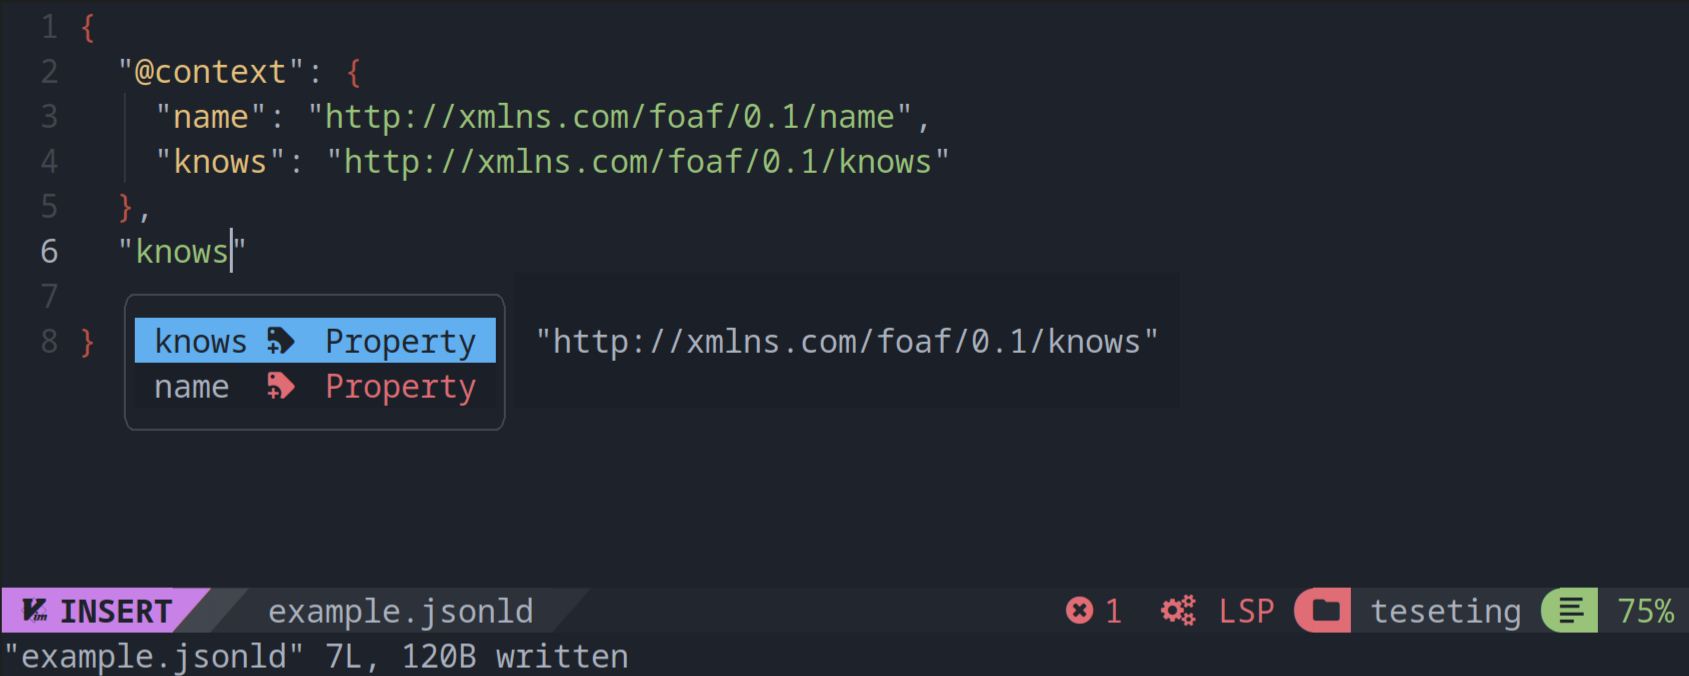
\includegraphics[width=.5\linewidth]{./fig/completion.png}
    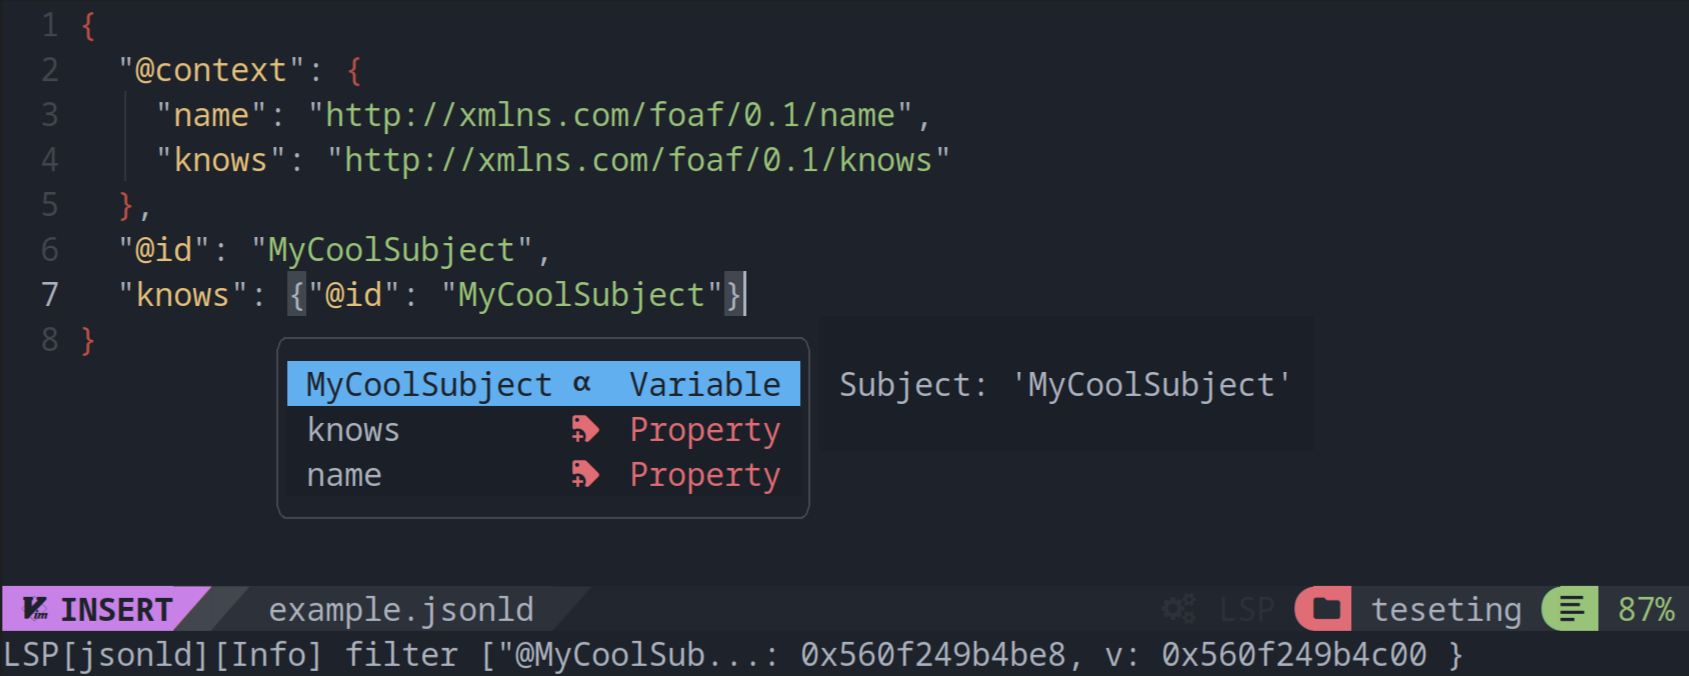
\includegraphics[width=.5\linewidth]{./fig/completion-id.png}
}
\caption{Screenshots showing completion functionality in NeoVim: left a list with all completion options, right a list containing the defined subject.}
\label{fig:complete}
\end{figure}


One of the key features of our LSP is code autocompletion based on the defined context. It extracts aliases from the inlined context, local contexts, and contexts hosted on the web. However, it currently does not take into account special context attributes such as context overloading or scoped contexts \cite{JSON-LD-W3C}. Figure \ref{fig:complete}, shoes this in action. The context defines two aliases, "name" and "knows". When the completion event is triggered, the user can choose between these aliases and the editor will complete the chosen alias. Defined subjects can be completed when writing \textit{@}, but will expand to more involved objects.

\begin{figure}
\centering
\makebox[\textwidth][c]{
    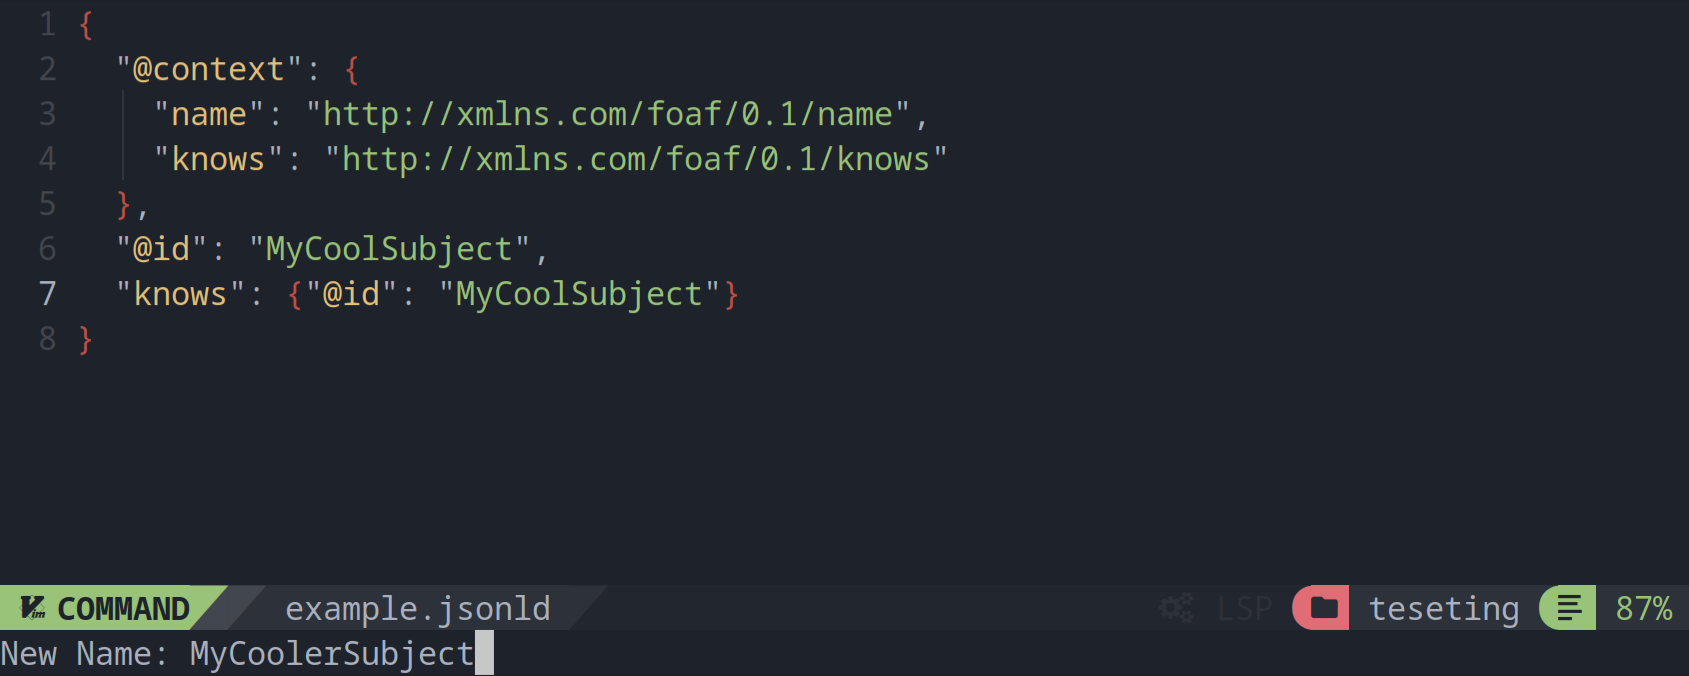
\includegraphics[width=.5\linewidth]{./fig/rename-1-small.png}
    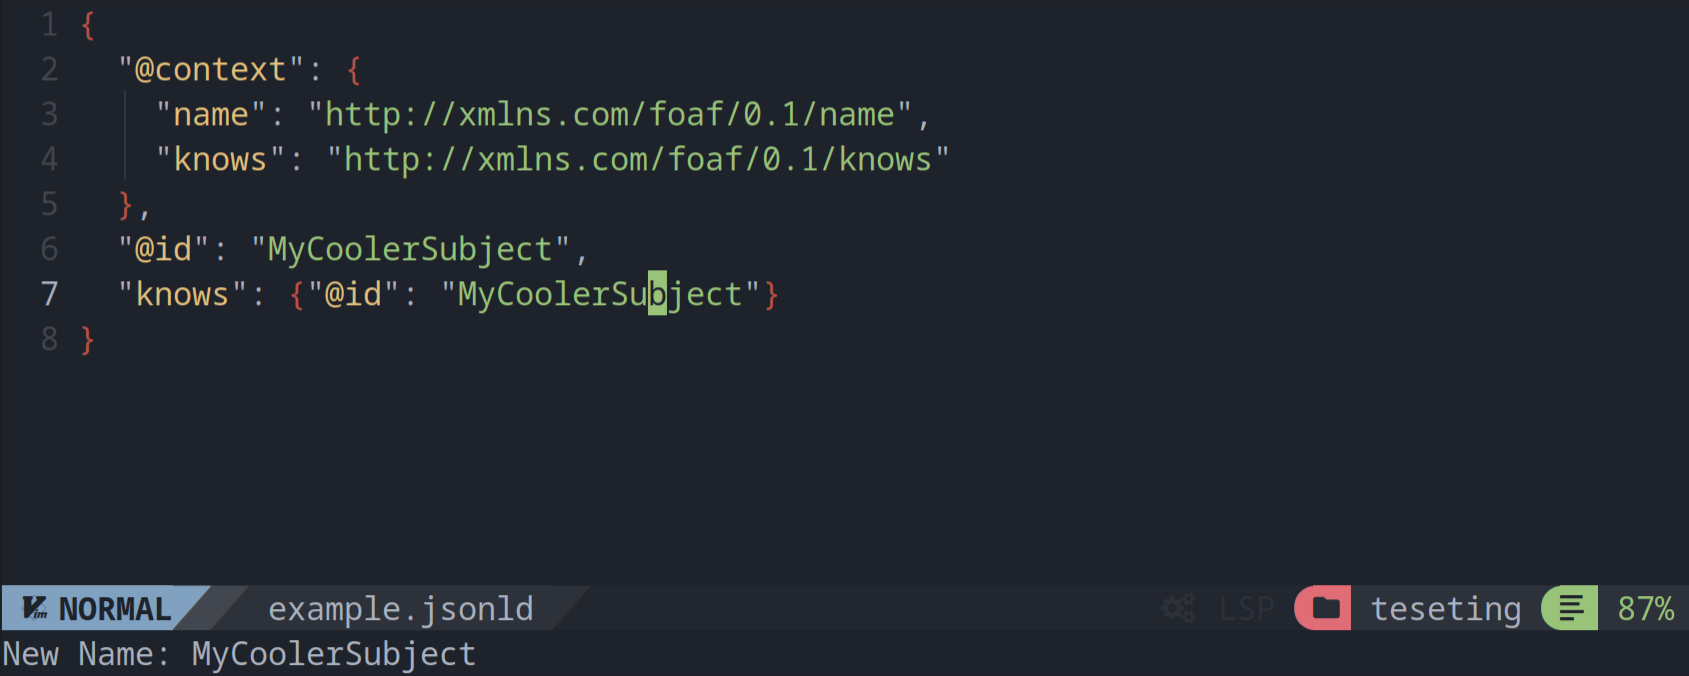
\includegraphics[width=.5\linewidth]{./fig/rename-2-small.png}
}
\caption{Screenshots showing renaming functionality in NeoVim: left NeoVim asks for the new name, right the subject is renamed.}
\label{fig:rename}
\end{figure}

Additionally, our LSP implementation supports renaming subjects. This is shown in Figure \ref{fig:rename}. The user is asked for the new name and the LSP server will respond with the required text changes that change all matching subjects to the new name.


% \section{Introduction}
%
% JSON-LD is a data serialization format that is used to describe semi-structured data on the web \cite{JSON-LD-W3C}.
% It adds semantic information to JSON, among others with the \textit{@context} property, pointing to a JSON-LD context.
% This context specifies how to map properties to predicates, called aliases.
% The \textit{@id} property then again specifies the subject of the current JSON object.
%
% JSON-LD allows you to write JSON and annotate the document with a context containing the necessary information for a JSON-LD processor to map it to RDF triples with IRIs.
% Writing this JSON becomes tedious when the context grows and not all properties are easy to remember.
% For example, just misspelling a JSON key can break your entire Linked Data use case.
%
% With its increasing popularity, contexts in JSON-LD also increase in complexity.
% For example, OSLO is an initiative in Flanders (Belgium) that is working to achieve interoperability by building semantic standards for different stakeholders such as government, industry and academia \footnote{\href{https://www.vlaanderen.be/digitaal-vlaanderen/onze-oplossingen/oslo}{OSLO} - Open Standaarden voor Linkende Organisaties}.
% Example JSON-LD context files for their vocabularies and application profiles \href{https://data.vlaanderen.be}{are available on the website data.vlaanderen.be}.
%
%
% Just like we use an editor when using functions and variables while programming, a semantic JSON-LD editor will be able to avoid common mistakes.
% In this demo, we show how a JSON-LD editor can help the developer experience.
% The Language Server Protocol (LSP) is a standard interface that separates the domain-specific logic from the editor's logic \cite{LSP-Multi}, allowing editors to offer advanced features such as code completion, hover information, and go-to-definition.
% By implementing an LSP for JSON-LD, developers can enjoy these advanced features and bring their editor's capabilities for JSON-LD up to par with programming languages.
%
% %% <!-- What is the competition doing? JSON with JSON schema? Autocompletion with Yasgui? Turtle lsp (stardog) -->
% Similar efforts have been made before, but never for JSON-LD. For example, the Yasgui editor\footnote{\href{https://triply.cc/docs/yasgui/}{Yasgui} - SPARQL editor}, a popular SPARQL human query interface, provides autocompletion based on the LOV API \cite{LOV}. Plugins can add autocompletion based on domain knowledge. These capabilities are built into the editor and can only be used with Yasgui.
% Stardog created open-source LSPs for turtle, TRIG, SPARQL, and more, however, they only concern themselves with correct syntax and keyword auto-completion \cite{stardog}. 
%
% Our demo JSON-LD LSP and installation instructions to use it with your favorite LSP capable editor can be found at \href{github.com/ajuvercr/jsonld-lsp](https://github.com/ajuvercr/jsonld-lsp}{github.com/ajuvercr/jsonld-lsp} (MIT).
%
%
% \section{Language Server Protocol}
%
% The Language Server Protocol (LSP) is a JSON RPC protocol developed by Microsoft to simplify the process of integrating language-specific logic into an editor \footnote{\href{https://microsoft.github.io/language-server-protocol/}{LSP} - Language Server Protocol}. 
% Prior to LSP, editors had to implement each programming language they wanted to support individually, resulting in an \(O(n*m)\) complexity where n is the number of editors and m is the number of programming languages.
% With LSP, editor and language-specific logic only needs to be implemented once, resulting in a much simpler \(O(n+m)\) complexity \cite{LSP-Multi}.
% LSP only concerns itself with the source files of the program and doesn't involve building, running, or debugging.
% This is in contrast to the Build Server Protocol \footnote{\href{https://github.com/build-server-protocol/build-server-protocol}{BSP} - Builder Server Protocol}.
%
% To implement an LSP, you can support predefined functions like autocompletion, rename, go to definition, find all references etc. Not everything needs to be implemented, as the editor and server can negotiate capabilities. For example, to support completion the server will respond to \textit{"textDocument/completion"} events, this event only contains the current cursor location, as document changes are communicated with other events. The server would respond with a completion list, containing visual labels for the user, and text edits that change the document when this completion item is selected. While initializing, the server would send a \textit{"client/registerCapability"} request to the client that informs the client of the completion capability. 
%
% Overall, the Language Server Protocol has greatly simplified the process of integrating language-specific logic into an editor \cite{LSP-editor}. LSP has made it easier for developers to work with a wide range of programming languages and editors. Currently, there exist over 130 LSP servers that cover 99 different programming languages. JSON-LD can be the 100th language to benefit from an LSP.

% \section{Demo}
%
% Our demo presents an implementation of a JSON-LD Language Server Protocol (LSP), developed using the Rust programming language and based on a basic LSP implementation \footnote{\href{https://crates.io/crates/tower-lsp}{Tower LSP} - Crate by Eyal Kalderon}. To extract predicate mappings from the context, we rely on the JSON-LD crate \footnote{\href{https://crates.io/crates/json-ld}{JSON-LD} - Crate by Timothée Haudebourg}. The full source code and installation instructions can be found on GitHub (MIT)\footnote{\href{https://github.com/ajuvercr/jsonld-lsp}{JSON-LD LSP} - Crate by Arthur Vercruysse}.
%
% \begin{figure}
% \centering
% \makebox[\textwidth][c]{
%     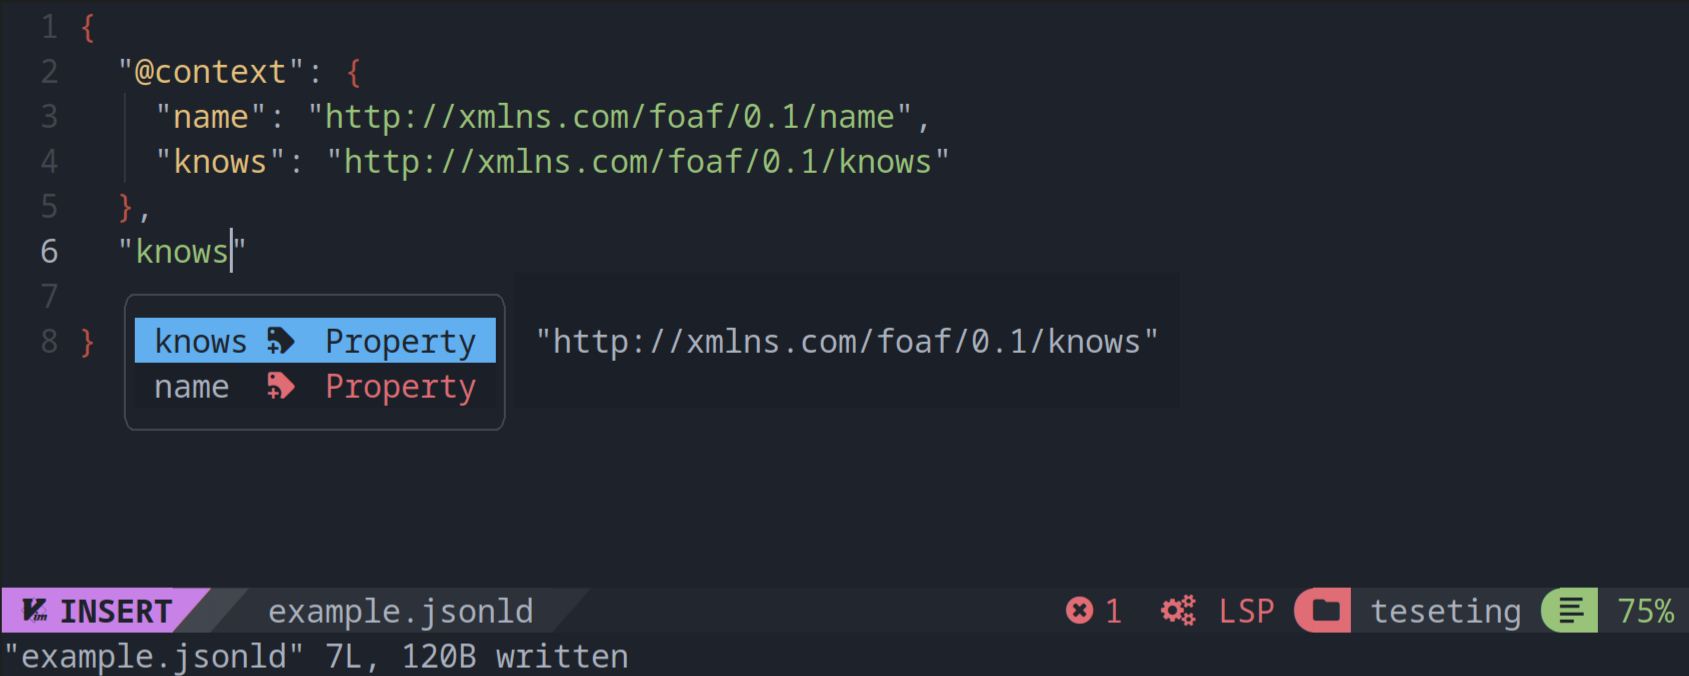
\includegraphics[width=.5\linewidth]{./fig/completion.png}
%     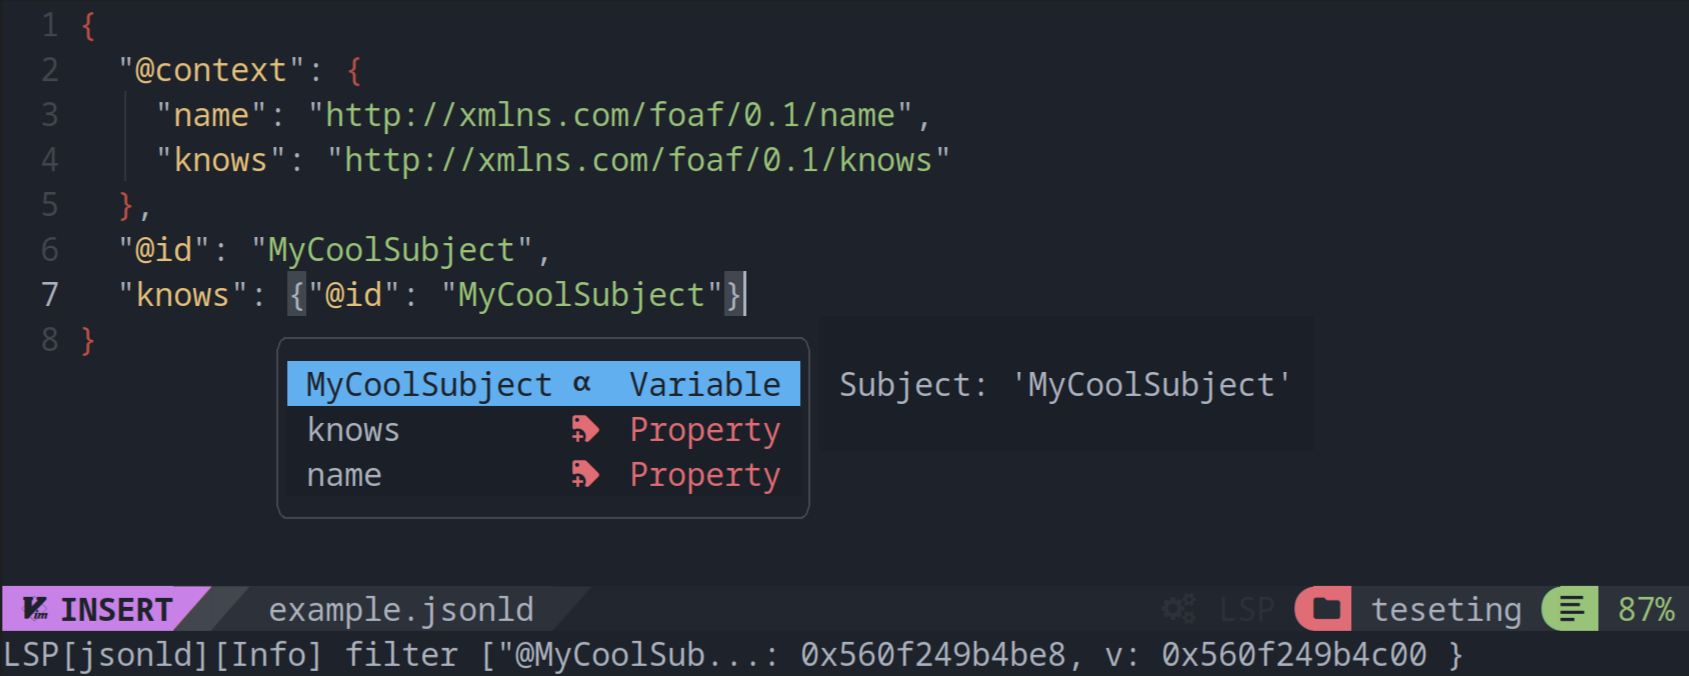
\includegraphics[width=.5\linewidth]{./fig/completion-id.png}
% }
% \caption{Screenshots showing completion functionality in NeoVim: left a list with all completion options, right a list containing the defined subject.}
% \label{fig:complete}
% \end{figure}
%
%
% One of the key features of our LSP is code autocompletion based on the defined context. It extracts aliases from the inlined context, local contexts, and contexts hosted on the web. However, it currently does not take into account special context attributes such as context overloading or scoped contexts \cite{JSON-LD-W3C}. In Figure \ref{fig:complete}, you can see this in action. The context defines two aliases, "name" and "knows". When the completion event is triggered, the user can choose between these aliases and the editor will complete the chosen alias. Defined subjects can be completed when writing \textit{@}, but will expand to more involved objects.
%
% \begin{figure}
% \centering
% \makebox[\textwidth][c]{
%     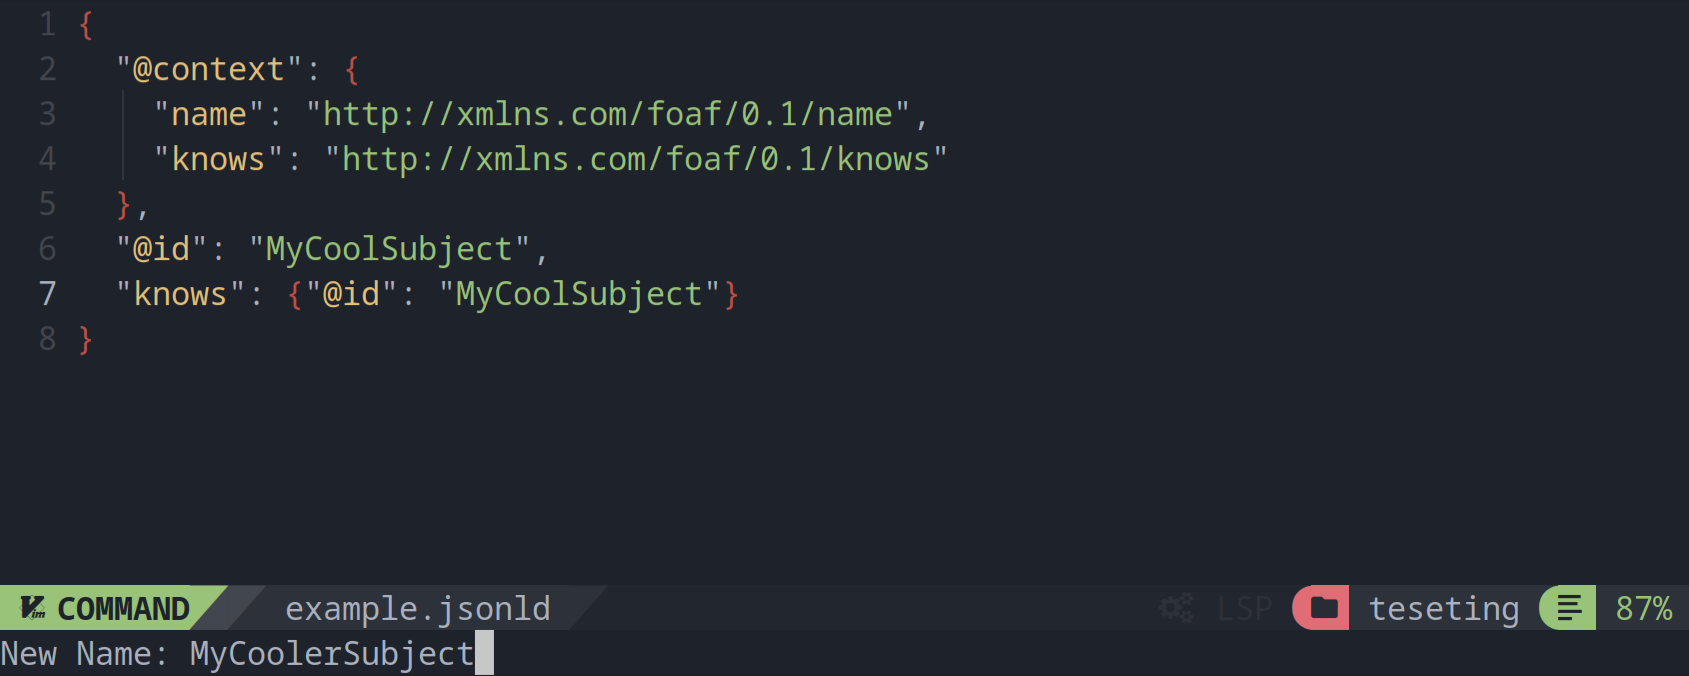
\includegraphics[width=.5\linewidth]{./fig/rename-1-small.png}
%     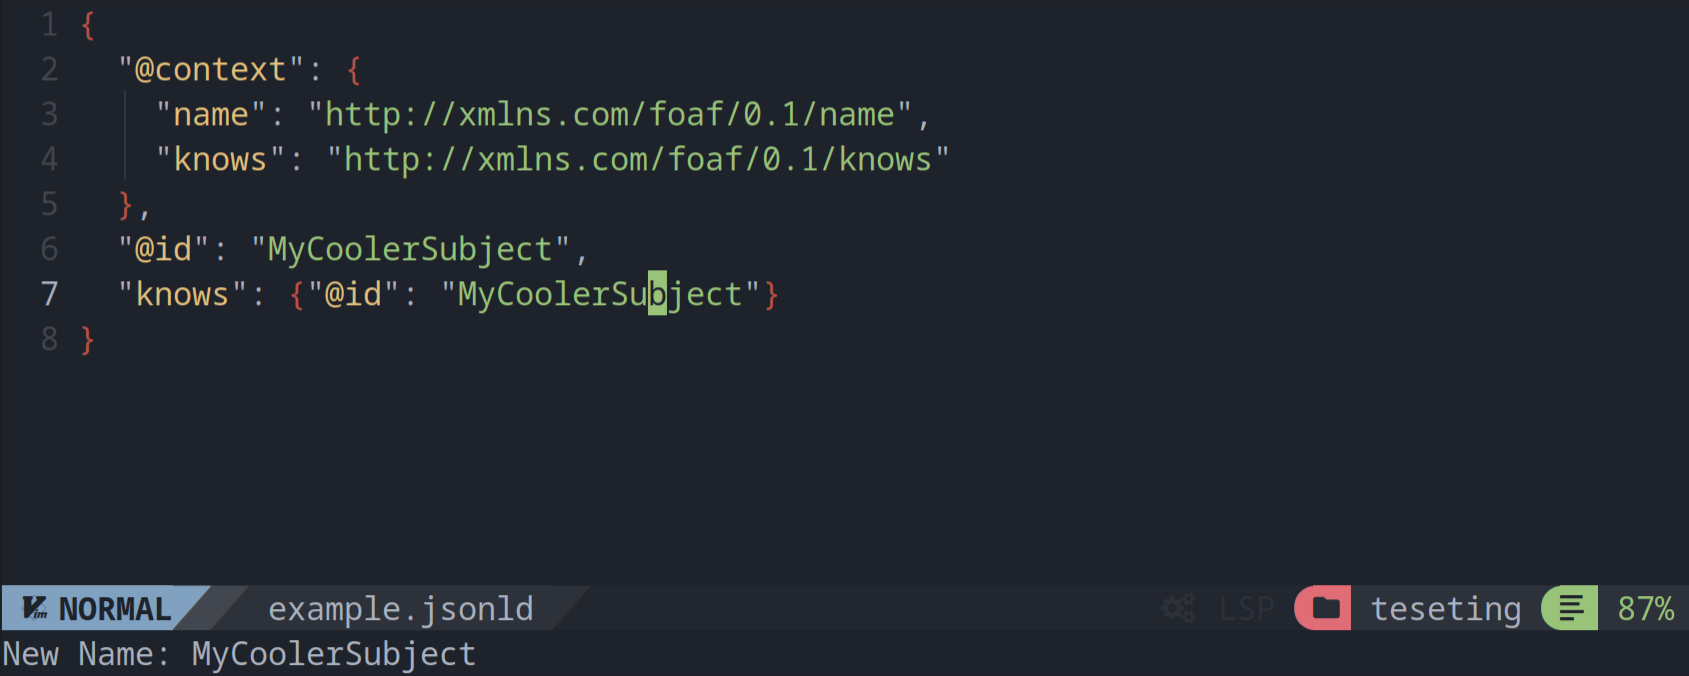
\includegraphics[width=.5\linewidth]{./fig/rename-2-small.png}
% }
% \caption{Screenshots showing renaming functionality in NeoVim: left NeoVim asks for the new name, right the subject is renamed.}
% \label{fig:rename}
% \end{figure}
%
% Additionally, our LSP implementation supports renaming subjects. This is shown in Figure \ref{fig:rename}. The user is asked for the new name and the LSP server will respond with the required text changes that change all matching subjects to the new name.


\section{Conclusion}

This demonstration merely scratches the surface of the vast capabilities of a JSON-LD LSP. By leveraging fully-interpreted contexts, the LSP can provide more contextually-relevant suggestions, taking into account context overloading and scoped contexts. Additionally, the LSP's functionality can be expanded to include the interpretation of referenced vocabularies, allowing completion for compacted predicates, like \textit{foaf:knows}. Despite its current limitations, the LSP already enhances the developer experience by facilitating the creation and editing of JSON-LD documents.

%%
%% The acknowledgments section is defined using the "acknowledgments" environment
%% (and NOT an unnumbered section). This ensures the proper
%% identification of the section in the article metadata, and the
%% consistent spelling of the heading.
% \begin{acknowledgments}
%   Thanks to the developers of ACM consolidated LaTeX styles
%   \url{https://github.com/borisveytsman/acmart} and to the developers
%   of Elsevier updated \LaTeX{} templates
%   \url{https://www.ctan.org/tex-archive/macros/latex/contrib/els-cas-templates}.  
% \end{acknowledgments}

%%
%% Define the bibliography file to be used
\jr{There is an issue in reference [3]}
\bibliography{bibliography}


\end{document}

%%
%% End of file

